\section{Hands-on examples for neural networks (1)}

As done for the parallel computing part, the next section will be a Jupyter Notebook which you can find on the E-Learning page of the course with the necessary modifications. Try and run it on Colab or on your local PC.

Before starting, two questions need to be answered: \textit{why do Neural Networks need to be deep? And what exactly is depth?} You can easily think of depth as the number of layers that are stack on top of each other in a NN, the more the deeper. The point is (as we shall see in our example) that if one NN is deeper than another with the same number of trainable parameters, it will be faster to train and will have better metric values. For really complicated and professional algorithms the difference in efficiency is more than relevant.

One last thing: the following \texttt{numpy} cheatsheet will be very useful in the following. Try to memorize it.

\begin{center}
    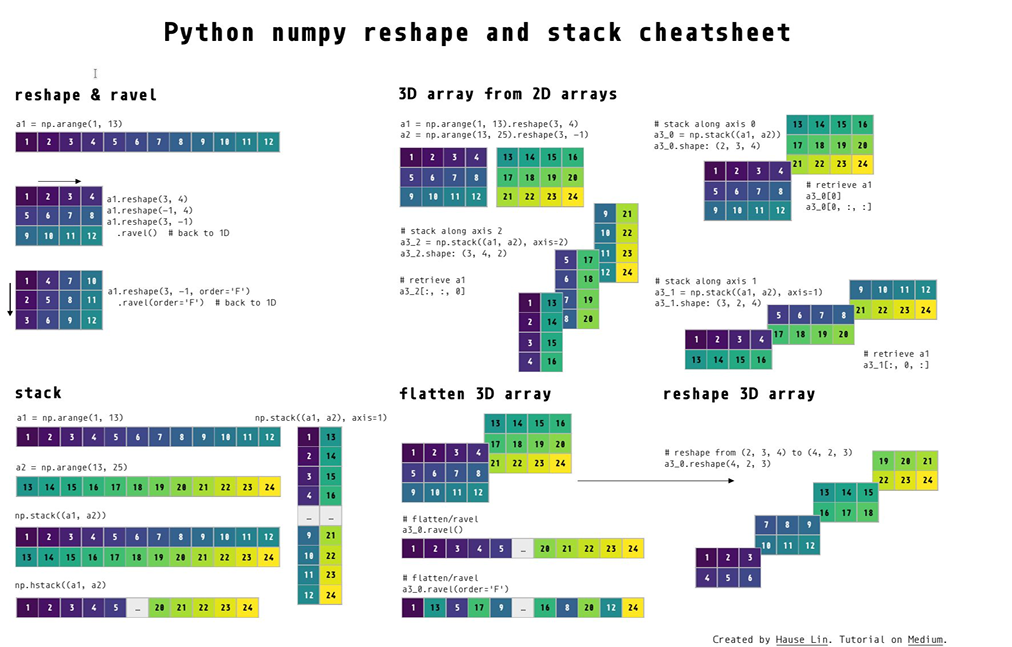
\includegraphics[width=\textwidth]{figuresML/lesson_ml_1_pag_999.png}
\end{center}

The first exercise consist of creating a simple classifier algorithm using an MLP and a DNN in order to compare their performances. In the second one you are required to build a regression algorithm by your own, so, even if the problem is already solved, you will find less guidelines and are encouraged to modify it and run it on your own. 

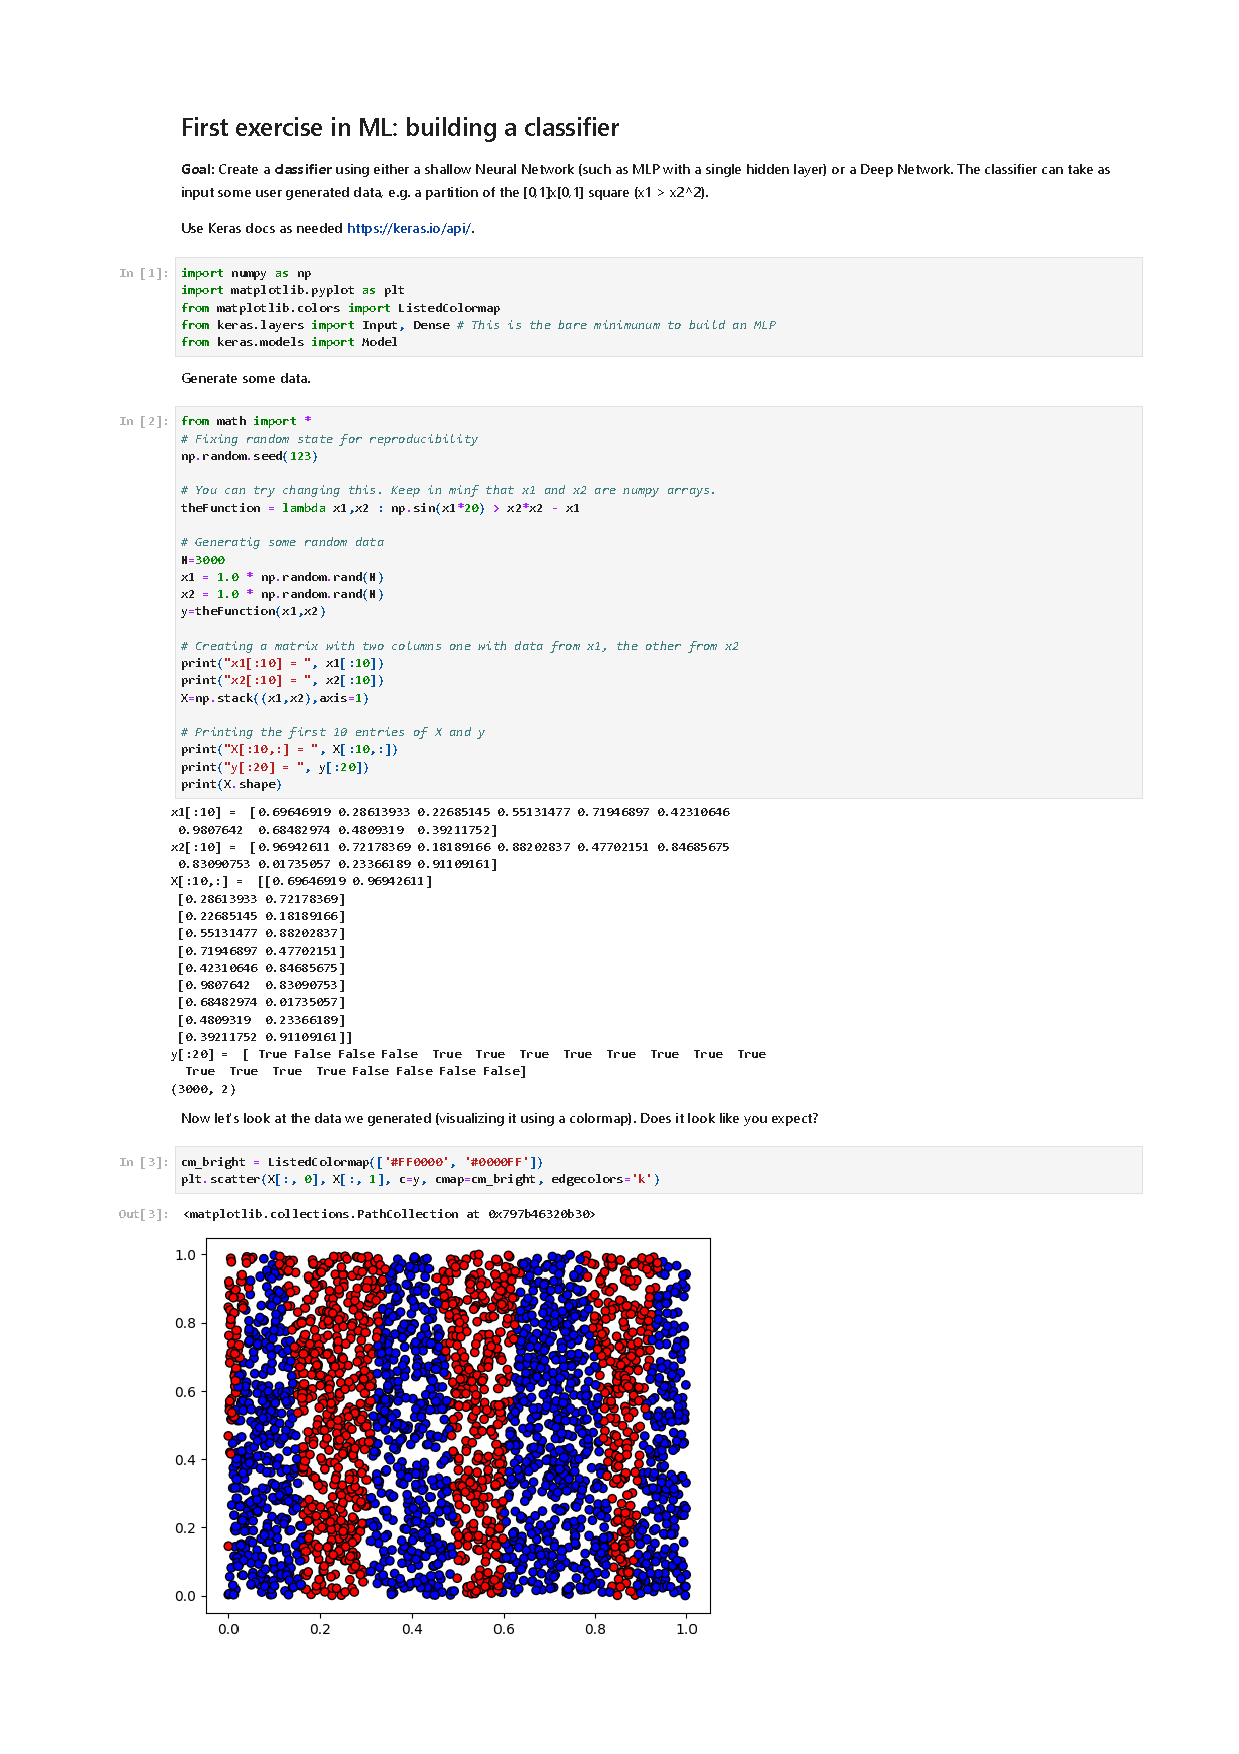
\includepdf[pages=-, pagecommand={\thispagestyle{plain}}]{lezioni/d_ML2A_SOL.pdf}

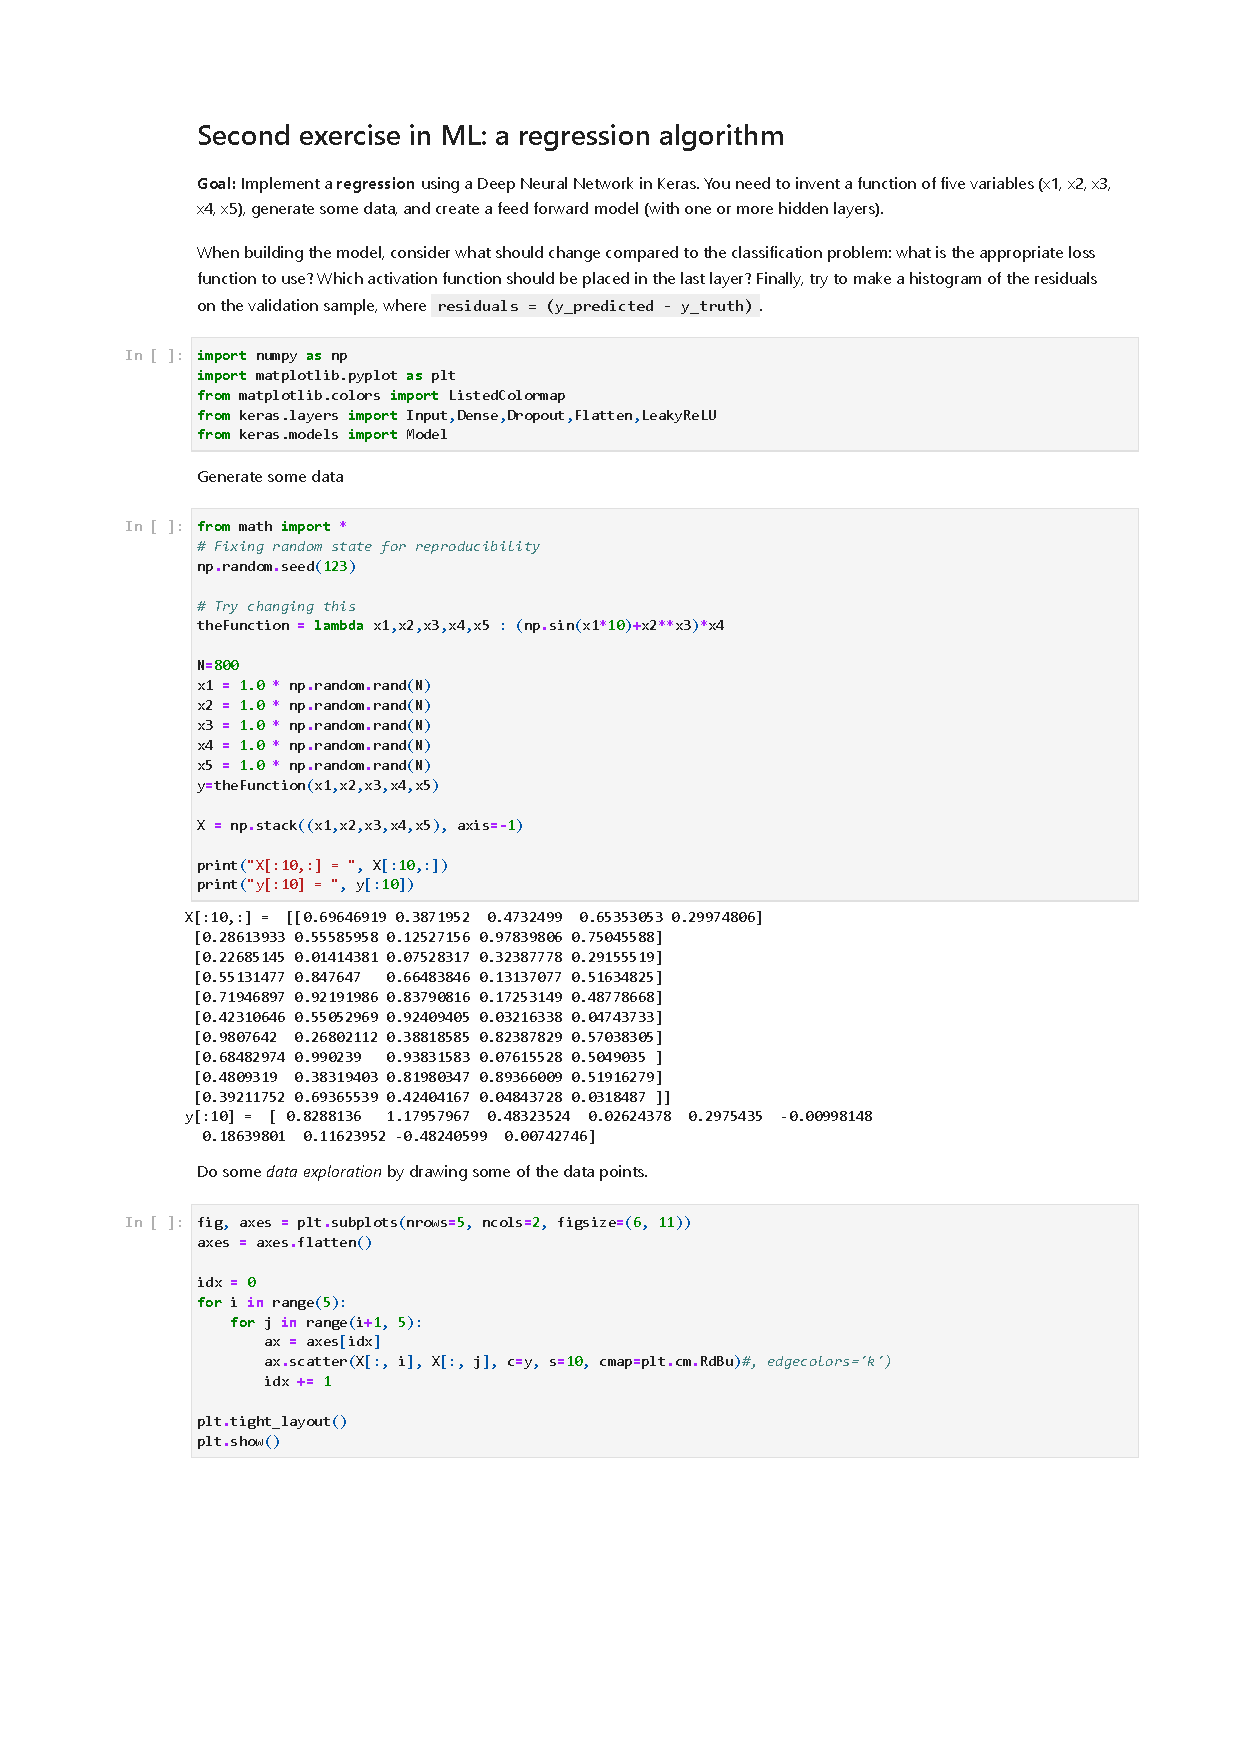
\includepdf[pages=-, pagecommand={\thispagestyle{plain}}]{lezioni/d_ML2B_SOL.pdf}
